\chapter{Implementation}

\section{CommLib}
\textbf{Author: Jeremy Sztavinovszki} 
The Communication Library, or CommLib for short is the part of the RECT stack, that handles all of the communication between the hosts over traditional protocols, like TCP, UDP and BLE.
This requires it to be especially performant. In order to avoid premature optimization however, the first part of this section on the implementation of the CommLib will only cover the first versions
of the code written to get the Library to work. After the first implementation there will be benchmarks and some profiling, in order to get a grasp on which aspects of the library need to be
optimized. The second section will then cover how these results were incorperated into designing a more polished version of the CommLib.

\subsection{Setting up the Library} 
The first steps of setting up the library are more or less the same as in any other rust project. First the project is initialized with \verb+cargo new --lib <rust-name>+. This creates a
new folder with the name specified in \verb+<library-name>+ and generates some files like Cargo.toml and src/main.rs. After this step is done the needed libraries for RECT are added to the
project through \verb+cargo add <dependency-name> -F <dependency-name>/<feature-name>+ these dependencies are the pulled and built by cargo (Rust's build tool) upon the initial build of the
project. The first iteration of the project then had the following dependencies:

\begin{itemize}
	\item tokio
	\item bluer
	\item anyhow
\end{itemize}

All in all the commands used to generate the CommLib project and install all dependencies looked like this:
\newline
\begin{minipage}{\textwidth}
	\begin{lstlisting}[language=bash, caption=Setup Commands for CommLib]
		cargo new --lib CommLib && cd CommLib
		cargo add tokio bluer anyhow -F tokio/full,bluer/full
		cargo build
	\end{lstlisting}
\end{minipage}

\subsection{First Implementation}
The first part of the implementation that was tackled was to create an abstraction layer over the existing protocols that RECT uses.
in order to have a nice and clean interface to work with and to avoid having to implement each feature separately for the
protocols. Of course, there was a bit of a problem with UDP because it is not meant to send structured data, so there is no feature parity between TCP and BLE.
between TCP and BLE and UDP in this respect, and UDP is only used to send unstructured data streams. To encapsulate the structured and unstructured data sent over the
and unstructured data sent over the common interface, there needs to be a way to convert the data, whether structured or not, into and from bytes in a way that is performant and has minimal overhead.
and has minimal overhead. In order to meet the above requirements, the following structure has been implemented.
 
\subsubsection{Messages and Packets}
% TODO Write about the packets and messages and maybe do a nice graphic.
% TODO find cite for TCP and UDP MTU 
The first thing taken into consideration for designing a data and class structure that is able to be sent over all of the protocols is the MTU's of the different protocols. 
For TCP and UDP the MTU, or maximum transmission unit, is defined by the Maximum Segment Size Option (MSS), which is technically limited to 65535 bytes (64KB), but as defined
in RFC 2675 \footcite{rfc2675} an MSS value of 65535 is defined to be interpreted as infinity and to be determined by Path MTU Discovery \footcite{rfc9293}. For BLE the MTU is 
defined by the L2CAP and can be anywhere from 23 to 65535, but the packet is fragmented and recombined by the L2CAP for transmission, which practically makes it infinite. % TODO find out why ble book cant be cited 

Another requirement for the interface was to be able to encapsulate the mechanism of sending a request to a peer and receiving a response. 
To do this, a pair of messages was implemented. This pair of messages, aptly named Request and Response, contains the data needed to make this work. This means 
that the request contains information about what topic to call on the remote machine, the data needed to fulfil that call, and an identification of the calling process, 
while the response contains the returned data and the ID of the client to which it should be returned. This identification is used to avoid confusion as to which process the data should be returned to, 
for example, when multiple processes are requesting data from the same remote service.

The identification mechanism used in the above case of sending data to a single recipient can also be adapted to send messages to multiple recipients.
The only adaptation required for the requesting and responding application to be able to send and receive broadcasts is to create a proxy object on the receiving side that acts as a single 
receiver to receive the data for multiple connections and then forward that data to all subscribing processes.  

The last use case covered by CommLib is the sending of a continuous stream of data. An example of this would be a sensor continuously sending data. To avoid the overhead of sending values over
protocols used in CommLib, it was decided to require a separate interface, e.g. a socket, that is used only for streaming the described data. This means that when the receiving side
is establishing a connection, it only needs to look at the identifier, e.g. the IP address, of the connected peer to decide which process to pass the data to, instead of reading a connection 
name from the packet sent, minimising the size of the packets that need to be sent. 

% TODO Write about the connection manager and also program that stuff
\subsubsection{The ConnectionManager}
The most important component in the whole CommLib is the ConnectionManager. It is a singleton object, which as the name would suggest manages all of the needed and used connections that are
requested by the client programs. Because the ConnectionManager is a singleton and because it must be able to handle being in concurrent execution environments the Rust borrow-checker has very
special requirements for how it is accessed. To meet these requirements the static variable holding the ConnectionManager singleton has needs to be wrapped in several objects to ensure it is
thread-safe, as well as making sure, that it is initialized and freed, when there are no references left to its smart-pointer. 

\begin{lstlisting}[language=Rust]
	pub static CONNECTION_MANAGER: Lazy<Arc<Mutex<ConnectionManager>>> =
	    Lazy::new(|| Arc::new(Mutex::new(ConnectionManager::new())));
\end{lstlisting}
Which leads to the above code, which has specifies, that the ConnectionManager is wrapped in the following types.

\begin{itemize}
	\item Lazy. This type allows any object held by it to be initialized only once and only when it is first called upon \footcite{once-cell-lazy}
	\item Arc. Arc stands for atomic reference counter and is a type of smart-pointer used in rust, when pointers need to be thread safe \footcite{rust-arc}
	\item Mutex. The mutex ensures, that only one process at a time can hold a reference to the held object in order to prevent issues such as race-conditions \footcite{tokio-mutex}
\end{itemize}

Any application using the CommLib needs to interact with this object in order to be able to use the communication methods provided by the library. But what functionality does the ConnectionManager provide?

\begin{itemize}
	\item Setting a connection to a database, which is used to read the connections configured by the clients.
	\item Receiving streams, requests and responses through any of the configured connections.
	\item Sending streams, requests and responses through any of the configured connections.
	\item Initiating an update of the connections, which checks changes in the configuration found in the database and the connections, that are currently active in the ConnectionManager.
\end{itemize}

% TODO Pretend you didn't already make everything railway programming and it still crashes because of stupid things.

\subsection{Profiling and Benchmarking}

\subsection{Polishing}

\subsection{Documentation}

\section{RECT Database}
\textbf{Author: Christoph Fellner}

\subsection{Why SQLite?}
The choice of a database system is a critical decision in the development of any application, and for RECT, the decision to use SQLite as the backend database 
is grounded in a thoughtful consideration of specific requirements tailored to the nature of small controllers.\newline

Given the diverse landscape of database systems, each with its unique set of advantages and drawbacks, a comprehensive evaluation of options is imperative. 
RECT's emphasis on catering to small controllers immediately guides the criteria for selecting a suitable database. Two key considerations emerge prominently: 
memory efficiency and self-containment.\newline

Small controllers typically operate within constrained resources, making memory efficiency a paramount concern. SQLite, renowned for its lightweight nature and 
minimal memory footprint, aligns seamlessly with this requirement. Its design prioritizes efficiency, ensuring optimal performance even in resource-limited 
environments.\newline

The self-contained nature of SQLite further contributes to its suitability for RECT's use case. Unlike some database systems that necessitate complex setup 
procedures and external dependencies, SQLite operates as a standalone, serverless database engine. This simplicity not only facilitates ease of use but also 
aligns with the desire to avoid intricate configurations. RECT benefits from a database solution that is straightforward to use and configure, enabling a 
seamless integration into the development workflow.\newline

While the focus on memory efficiency and self-containment narrows down the pool of potential databases, SQLite emerges as an optimal choice that strikes a 
balance between these requirements. The careful consideration of these factors positions SQLite as a reliable and pragmatic choice for RECT, providing the 
necessary functionality without introducing unnecessary complexity.\newline

In conclusion, the selection of SQLite for RECT's backend database is a result of a meticulous comparison of different options, with a keen focus on the 
specific needs of small controllers. The prioritization of memory efficiency, self-containment, and ease of use collectively affirm SQLite as the ideal database 
solution, ensuring optimal performance and simplicity in the context of RECT's development environment.

\subsubsection{SQLite}
SQLite\footcite{sqlite} stands out prominently as a frontrunner when it comes to selecting a memory-efficient database, and for good reasons. As a small, fast, 
and serverless database engine, SQLite aligns perfectly with the requirements of applications like RECT, particularly those designed for small controllers.\newline

The serverless nature of SQLite is a noteworthy feature. Unlike some database systems that necessitate a separate server process for operation, SQLite operates 
in a self-contained manner. This characteristic not only simplifies deployment and configuration but also contributes to its efficiency and suitability for 
resource-constrained environments.\newline

\paragraph{History}
Originally developed in the year 2000 by D. Richard Hipp for the US Army, SQLite has evolved into an open-source database engine. Its implementation in the C 
programming language renders it highly portable, allowing it to run seamlessly on a myriad of platforms. This broad compatibility makes SQLite an excellent 
choice for applications that need to be deployed across diverse environments.\newline

\paragraph{Compatibility with Rust}
The compatibility between SQLite and Rust is facilitated through the rusqlite library, providing a native and ergonomic interface for Rust developers to 
interact with SQLite databases. This seamless integration ensures that the benefits of SQLite, such as its speed and efficiency, can be harnessed effortlessly 
within Rust projects.\newline

Moreover, SQLite offers the flexibility to store the database in memory, enabling rapid access and retrieval of data. The asynchronous access to SQLite 
databases further enhances its versatility, allowing applications like RECT to efficiently manage and interact with data in an asynchronous programming paradigm.\newline

In essence, SQLite's combination of speed, efficiency, serverless operation, and broad platform compatibility positions it as an ideal choice for applications 
that prioritize memory efficiency. For RECT, SQLite, with its inherent qualities and compatibility with Rust through rusqlite, emerges as a robust and fitting 
solution for the backend database, contributing to the overall efficiency and performance of the application.

\subsubsection{PostgreSQL}
Postgres\footcite{postgres}, also known as PostgreSQL, stands as a widely adopted backend database for web applications and websites. Renowned for its robust 
features and scalability, PostgreSQL operates on a client/server architecture, where the database is managed by a dedicated server process. This architecture 
allows multiple clients to interact with the database concurrently, even when accessing the same data simultaneously. The inherent support for handling multiple 
clients makes PostgreSQL particularly well-suited for scenarios where asynchronous access to the database from multiple threads is crucial.\newline

\paragraph{History}
The origins of PostgreSQL trace back to the Berkeley Computer Science Department at the University of California in 1986. Initially named Postgres, the project 
evolved over time and eventually became known as PostgreSQL, although the colloquial shortening to Postgres is still common. In 1996, the project transitioned 
to an open-source model, relying on the contributions of a dedicated group of volunteers for maintenance and improvement. Operating seamlessly on major 
operating systems, PostgreSQL has garnered a reputation for its reliability and adherence to standards.\newline

\paragraph{Compatibility with Rust}
In the realm of Rust, PostgreSQL finds compatibility through the rust-postgres library, which provides a native interface for Rust developers to interact with 
PostgreSQL databases. The integration of Rust and PostgreSQL is further optimized for asynchronous programming through the tokio-postgres library. This library, 
built on top of Tokio, enhances the performance of asynchronous interactions with PostgreSQL databases via Rust, making it well-suited for modern, concurrent 
application scenarios.\newline

The client/server architecture of PostgreSQL, coupled with its robust Rust libraries, positions it as a formidable choice for applications that require a 
backend database with support for concurrent access and asynchronous operations. While it may have started as a project nearly four decades ago, PostgreSQL 
continues to evolve and thrive, maintaining its relevance in the dynamic landscape of web development and database management.

\subsubsection{MySQL}
MySQL\footcite{mysql} has established itself as a heavyweight in the realm of backend databases, with giants like YouTube, Facebook, and Twitter relying on its 
robust capabilities. Widely utilized for storing data from web services, MySQL operates on a client/server architecture similar to PostgreSQL, featuring a 
singular server process managing the database and facilitating access for multiple clients.\newline

\paragraph{History}
The MySQL project traces its roots back to 1994 when Michael Widenius and David Axmark initiated its development. Initially conceived as a fork of the mSQL 
database, MySQL underwent a significant transformation and was eventually rewritten from scratch. Since 2010, MySQL has been under the development umbrella of 
Oracle. While the project remains open-source, Oracle also offers an enterprise version of MySQL with additional features and support.\newline

In response to concerns about the direction of MySQL's development under Oracle, the original developers embarked on a new venture called MariaDB. This project 
represents a fork of MySQL and maintains full compatibility with its predecessor. The availability of MariaDB provides users with an alternative that adheres 
to the principles of open-source development.\newline

\paragraph{Compatibility with Rust}
For Rust developers seeking to interface with MySQL, the mysql library, complemented by an extension called \verb+mysql_async+, offers a convenient and native 
Rust interface. The \verb+mysql_async+ library, built on the Tokio framework, specifically caters to asynchronous client access, aligning with modern 
programming paradigms that emphasize concurrent and non-blocking operations.\newline

In summary, MySQL's widespread adoption by major players in the tech industry underscores its reliability and scalability as a backend database. The project's 
history, marked by its evolution under different entities, has given rise to alternative options such as MariaDB. The existence of Rust libraries like mysql 
and \verb+mysql_async+ further enhances MySQL's accessibility and usability within the Rust programming ecosystem, enabling developers to seamlessly integrate 
MySQL into their applications.

\subsubsection{Comparison}
The table provides a concise comparison of key features among SQLite, PostgreSQL, and MySQL, shedding light on their architectural, compliance, support, and 
use-case distinctions:

\begin{center}
    \begin{tabular}{ | m{3cm} | m{4cm}| m{4cm} | m{4cm} | } 
      \hline
      Features & SQLite & PostgreSQL & MySQL \\ 
      \hline
      Architecture & File Based (Self-contained) & Client/Server & Client/Server \\ 
      \hline
      ACID Compliance & Always & Always & Only with InnoDB and NDB Cluster storage engines \\ 
      \hline
      In-memory Support & Yes & No & Yes \\
      \hline
      Editions & Community (Free) with option of pro support & Community with option of commercial support & Community, Standard, and Enterprise \\
      \hline
      Popular Use-cases & Low-Medium Traffic Websites, IoT and Embedded Devices, Testing and Development & Analytics, Data Mining, Data Warehousing, Business Intelligence, Hadoop & Web Sites, Web Applications, LAMP stack, OLTP-based applications \\
      \hline
      Key Customers & Adobe, Facebook, and Apple & Cloudera, Instagram, and ViaSat & GitHub, Facebook, and YouTube \\
      \hline
    \end{tabular}
\end{center}

This comparison underscores the diverse strengths and use cases of each database system. SQLite's file-based, self-contained architecture makes it suitable for 
low to medium traffic websites, embedded devices, and development environments. PostgreSQL, with its client/server architecture and robust feature set, caters 
to analytics, data mining, warehousing, and business intelligence needs. MySQL, available in various editions, is widely employed in web applications, LAMP 
stack environments, and OLTP-based applications. Each database system has its own unique advantages, making the selection contingent on the specific 
requirements and scale of the intended use.\newline

After we looked into the three possiblyties mentioned above we created an enviroment to benchmark the different databases. We used docker to create a container for each 
database and then ran a benchmark test on each of them. The benchmark test was a simple test that inserted 1000 rows into a table and then read them again. The benchmark is
purposefully simple, because we won't be using the database for complex queries. More about the benchmark tests can be found \href{tests.tex}{here}.

\subsection{Database Structure}

The RECT Database is designed like \ref{fig:db-architecture}. This is a Entity Relationship Diagram (ERD) that shows the structure of the database. The database implements a
classic star schema, with the connections table as the center of the star. The connections table is linked to the client, method and address tables.

\begin{figure}
	\centering

	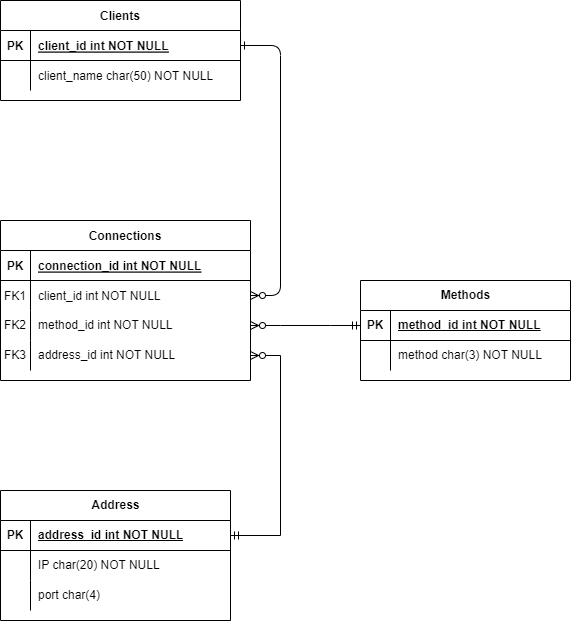
\includegraphics[width=\textwidth]{img/RECT-erd}

	\caption{Database Architecture of RECT.}
	\label{fig:db-architecture}
\end{figure}



The RECT database is structured according to the widely adopted star model, providing a robust framework for efficiently managing connection data. Comprising four distinct 
tables, namely connections, client, method, and address, this database architecture ensures comprehensive organization and accessibility of critical information.\newline

The connections table serves as a central hub, linking to the other three tables through their respective IDs and storing unique identifiers for each connection. 
Meanwhile, the client table houses data pertaining to the clients associated with specific connections, facilitating targeted access to connection information. In the 
method table, precisely three objects—BLE (Bluetooth Low Energy), TCP (Transmission Control Protocol), and UDP (User Datagram Protocol)—are stored, representing the 
available connection types within the RECT ecosystem. Additionally, the address table stores essential network information, including IP addresses and ports, with the 
provision for a null port value in instances where the connection method is BLE.\newline

By adopting this schema, the RECT database optimizes accessibility to connection data for clients by establishing seamless linkages between tables. Leveraging the Rusqlite
library, the backend components can efficiently query and retrieve pertinent information, enabling effective communication over the designated connections. Moreover, this 
database structure facilitates the extraction of various insights and metrics, empowering users to select and analyze data such as:

\begin{itemize}
  \item[] How many BLE, TCP or UDP connections are available?
  \item[] All connections of a specific client.
  \item[] All clients that have a specific connection.
  \item[] All connections that are available.
  \item[] How many connections are available in total?
  \item[] Are there more connections to the same client?
\end{itemize}

\subsection{Database usage}

The RECT Database serves as a pivotal resource accessible not only to the Rust Interface but also to the entirety of the backend infrastructure within the RECT stack. 
Acting as the backbone for data management, the Rust Interface undertakes the essential task of configuring the database, a process that includes the insertion of data 
sourced from the JSON file into its tables. This data encompasses a comprehensive inventory of available connections tailored specifically for the local RECT Client system.
Each connection within this dataset is meticulously characterized by a unique identifier, a designated communication method (be it BLE, TCP, or UDP), and a corresponding 
address composed of an IP address and port number.\newline

Upon completing the database setup and population with pertinent connection data, the backend components of the RECT stack rely on this repository to establish and manage 
communication channels. However, before the backend can effectively harness the capabilities of the database, the Rust Interface must first initialize the database setup 
and meticulously inject the JSON-derived information. Following this preparatory phase, the Interface seamlessly facilitates backend access to the database via the CommLib,
thereby ensuring a streamlined pathway for communication. Subsequently, armed with access to this centralized database, the backend components adeptly navigate and utilize
the provided connections to facilitate efficient communication processes tailored to the demands of the RECT ecosystem.

\section{Rust Interface}
\textbf{Author: Christoph Fellner}
One of the main sections of the RECT project is the Rust Interface. The Rust Interface is the part of the RECT stack that is responsible for the communication between 
the different parts of the stack. That means that the Rust Interface is responsible for the communication between the CommLib and the RECT Database. The RECT Database is 
part of the Rust Interface, it stores Data about all available RECT connections. The Rust Interface also communicates with the Python Service and the C++ Service. So 
basically the Rust Interface it responsible for the communication between the frontend and the backend of the RECT stack.\newline

In order to achieve this functionality the first step was to create a Rust module for gRPC communication. The gRPC communication is done with the help of the tonic library.
The tonic library is a gRPC library for Rust, which is based on the tokio library. The tokio library is a runtime for writing reliable asynchronous applications with Rust.
The gRPC module is responsible for the communication between the Rust Interface and the Python Service and the C++ Service. The gRPC module is also responsible for the 
communication between the Rust Interface and the CommLib.\newline 

The second step was to create a module for the RECT Database. The RECT Database is a in-memory SQLite database. The module uses the rusqlite library with the addition of
the tokio-rusqlite library. The tokio-rusqlite library is a asynchronous version of the rusqlite library. The Rust Interface implements the RECT Database, creates the 
necessary tables and provides the necessary functions to communicate with the database. The module is also responsible for the inserts of the available connections from a
JSON file into the database. The JSON file is created by the frontend and contains all available connections for the RECT stack.\newline

For the second step to work the Rust Interface also needs to be able to read the JSON file. The JSON file is read by another module of the Rust Interface. The module uses
the serde library to read the JSON file. The serde library is a framework for serializing and deserializing Rust data structures efficiently and generically. The module 
defines suitable structures for the data strored in the JSON file and then reads the file and stores the data in the defined structures. The database module then takes
this data and stores it in the RECT database.\newline

With these modules completed the Rust Interface is able to communicate with the CommLib, the Python Service and the C++ Service. In conclusion, the Rust Interface plays a 
crucial role within the RECT project, facilitating communication between various components of the stack. Through the implementation of modules for gRPC communication and 
the RECT Database, the Rust Interface ensures seamless interaction between the frontend and backend elements. Leveraging libraries such as tonic, tokio, rusqlite, and 
serde, the interface achieves reliable and efficient communication, handling tasks such as database management and data serialization effectively. Overall, the Rust 
Interface serves as a vital bridge, enabling smooth operation and integration within the RECT stack.

\section{Rust Service}
\subsection{Documentation}

\section{C++ Implementation}
\textbf{Author: Maximilian Dragosits}
The C++ Implementation is one of the two outward facing components of the RECT stack. Alongside the Python Implementation 
it serves as a library in order for developers to be able to create robots, that are able to communicate with each other, much
easier then before. This is accomplished by abstracting most of the complexities of gRPC behind the \textit{Rectcpp} class. 

The class only needs to be initialized with IP-Addresses for the different services that it offers and be given the IP of 
another of its kind and then it should be a simple act of using the predefined methods within the class in order to 
effortlessly communicate with other robots or devices running this or the Python frontend implementation.

\subsection{Rectcpp class}
\subsection{Documentation}

\section{Python Implementation}

\subsection{Documentation}

\section{Implementation Comparison}

\filbreak
